% This is "sig-alternate.tex" V2.0 May 2012
% This file should be compiled with V2.5 of "sig-alternate.cls" May 2012
%
% This example file demonstrates the use of the 'sig-alternate.cls'
% V2.5 LaTeX2e document class file. It is for those submitting
% articles to ACM Conference Proceedings WHO DO NOT WISH TO
% STRICTLY ADHERE TO THE SIGS (PUBS-BOARD-ENDORSED) STYLE.
% The 'sig-alternate.cls' file will produce a similar-looking,
% albeit, 'tighter' paper resulting in, invariably, fewer pages.
%
% ----------------------------------------------------------------------------------------------------------------
% This .tex file (and associated .cls V2.5) produces:
%       1) The Permission Statement
%       2) The Conference (location) Info information
%       3) The Copyright Line with ACM data
%       4) NO page numbers
%
% as against the acm_proc_article-sp.cls file which
% DOES NOT produce 1) thru' 3) above.
%
% Using 'sig-alternate.cls' you have control, however, from within
% the source .tex file, over both the CopyrightYear
% (defaulted to 200X) and the ACM Copyright Data
% (defaulted to X-XXXXX-XX-X/XX/XX).
% e.g.
% \CopyrightYear{2007} will cause 2007 to appear in the copyright line.
% \crdata{0-12345-67-8/90/12} will cause 0-12345-67-8/90/12 to appear in the copyright line.
%
% ---------------------------------------------------------------------------------------------------------------
% This .tex source is an example which *does* use
% the .bib file (from which the .bbl file % is produced).
% REMEMBER HOWEVER: After having produced the .bbl file,
% and prior to final submission, you *NEED* to 'insert'
% your .bbl file into your source .tex file so as to provide
% ONE 'self-contained' source file.
%
% ================= IF YOU HAVE QUESTIONS =======================
% Questions regarding the SIGS styles, SIGS policies and
% procedures, Conferences etc. should be sent to
% Adrienne Griscti (griscti@acm.org)
%
% Technical questions _only_ to
% Gerald Murray (murray@hq.acm.org)
% ===============================================================
%
% For tracking purposes - this is V2.0 - May 2012

\documentclass{sig-alternate}
\usepackage{hyperref}
\begin{document}

\conferenceinfo{OpenSym}{'14 Aug 27-29 2014, Berlin, Germany}
\CopyrightYear{2014}
\crdata{978-1-4503-3016-9/14/08}
%\crdata{http://dx.doi.org/10.1145/2641580.2641624}

\title{Drupal as a Commons-Based Peer Production community: a sociological perspective}

\numberofauthors{1}
\author{
% You can go ahead and credit any number of authors here,
% e.g. one 'row of three' or two rows (consisting of one row of three
% and a second row of one, two or three).
%
% The command \alignauthor (no curly braces needed) should
% precede each author name, affiliation/snail-mail address and
% e-mail address. Additionally, tag each line of
% affiliation/address with \affaddr, and tag the
% e-mail address with \email.
%
% 1st. author
\alignauthor
David Rozas\\
       \affaddr{Centre for Research in Social Simulation}\\
       \affaddr{Department of Sociology}\\
       %\affaddr{Faculty of Arts and Human Sciences}\\
       \affaddr{University of Surrey}\\
       %\affaddr{Guildford, Surrey, GU2 7XH, United Kingdom}\\  
       \affaddr{United Kingdom}\\     
       \email{drozas@surrey.ac.uk}
}

\maketitle
\begin{abstract}
%THIS SHOULD BE NO MORE THAN 100 WORDS
The aim of this research consists of extracting a set of insights related to the dynamics, group decision making procedures, motivations to contribute and mechanisms employed in the coordination of Commons-Based Peer Production communities, using as a case study the community responsible for the development of the Free/Libre Open Source Software Drupal. A sociological perspective is taken for this purpose, and a set of social research qualitative and quantitative methods employed for the study of online communities (virtual ethnography) are being used.  
\end{abstract}


\keywords{Commons-Based Peer Production, Free/Libre Open Source Software, Drupal, Virtual Ethnography, Activity Theory} % NOT required for Proceedings

\section{Overview}
Drupal is a free software content management framework currently employed in nearly 2\% of the websites worldwide\footnote{Statistics from W3Techs accessed on May 2014 (\url{http://w3techs.com/technologies/overview/content_management/all})}.
  With more than 1 million users registered at Drupal.org, more than 30.000 source code contributors and hundreds of local, national and international Face to Face (F2F) events  being held worldwide, the Drupal community represents one of the most vibrant examples of the success of Free/Libre Open Source Software (FLOSS). The expansion of some of the FLOSS principles and modes of production into other areas such as collaborative creation, hacklabs, P2P economy, etc. is attracting the attention of many researchers from several disciplines. Benkler\cite{benkler2006wealth} coined the term Commons-Based Peer Production (CBPP) to describe a new model of socio-economic production in which groups of loosely connected individuals cooperate with each other to produce meaningful products without a traditional hierarchical organisation, usually with the help of low cost integration mechanisms, such as the Internet. Due to the expansion of CBPP into further areas of knowledge, this phenomenon becomes of even greater interest. There have been several calls to promote a better dialogue between FLOSS and the social sciences in order to identify new theories and research designs \cite{VonKrogh2007}. There is as well a growing interest in the study of Drupal and its community from diverse disciplines. However, the Drupal community is a relatively young one. Therefore, these efforts are quite recent, and many aspects remain to be explored.

The aim of this research is to shed light on the dynamics, principles, motivations and mechanisms employed in the coordination of CBPP communities, by exploring the Drupal community as a case study.  This  will allow the extraction of insights related to the dynamics, group decision making procedures, motivations to contribute and mechanisms employed in the coordination of this community. The study is being carried out following a virtual ethnographic perspective\cite{hine2000virtual}, which adapts traditional ethnographic methods for the study of online communities and their cultures. A triangulation of qualitative and quantitative methods such as participant-observation, content analysis, interviews and surveys will be used to achieve this goal.

\section{Activity theory as a framework to explore collaboration}
Activity theory (AT) is a framework which sets the activity as the unit of analysis in the study of human activities. The use of AT as a lens to understand the dynamics of the Drupal community, provides a powerful tool which incorporates the notions of mediation and historical analysis, allowing a contextual study of the practices and emergence of structures, as pointed out by Uden et al.\cite{Uden2007} in their call to use AT for the study of FLOSS communities. Instead of focusing only on the individual, the interactions between the subject, the artifacts and the rest of individuals under certain organisational settings can be explored. The second generation of AT proposed by Engestr{\"o}m\cite{engestrom1987learning} extended the original conceptualisation, incorporating the rules that regulate the activity, the community sharing the interest and the division of labour. The model is usually represented as a triangle with six interrelated elements and the outcome of the activity. As an illustration of its application as framework, I describe the conceptualisation of the process of creation of contributed modules in Drupal. Contributed modules are sets of source code files written by members of the Drupal community which provide new functionalities that are not part of the core of the system.

\begin{itemize}
	\item \textit{Subject(s)}: the developer(s) responsible of the development and maintenance of the contributed module (maintainers).
	\item \textit{Instruments}: the coordination tools employed by the maintainers and the rest of members of the community. A typical example of instrument would be the issues list associated with each module project page.
	\item \textit{Object}: the module developed as a result of the activity.
	\item \textit{Rules}: the explicit and implicit rules which regulate the development of the module. Examples of explicit rules are the coding standards agreed by the community for the modules or the guidelines for the contribution, while examples of implicit rules are the criteria employed by maintainers for the evaluation of contributions from other members without permissions to perform modifications in that module. 
	\item \textit{Community}: the members of the Drupal community. The interaction with a concrete module is typically due to the fact that they are users of it. They can make use of the instruments to provide feedback about it, request new features, contribute patches to solve bugs or extend its functionalities, etc. 
	\item \textit{Division of labour}: it represents the distribution of tasks for the development of the module. An example of a form of division of labour is the allocation of tasks according to the different skills of the members, using the issues list as instrument.
\end{itemize}

Figure \ref{drupal_module_at} summarises the relationships between all the entities using the triangular model of the second AT generation. The use of AT as analytical framework will allow us to understand how the process is organised and to explore what social practices and relationships operate in this context. For example: how are contributions (e.g.: submission of a patch, feature request, etc.) from other members of the community evaluated by the maintainer(s) and why are they accepted or rejected? Is there any impact of other instruments (e.g: an evaluation of the user profile) as part of the decision-making process?

\begin{figure}
	\centering
	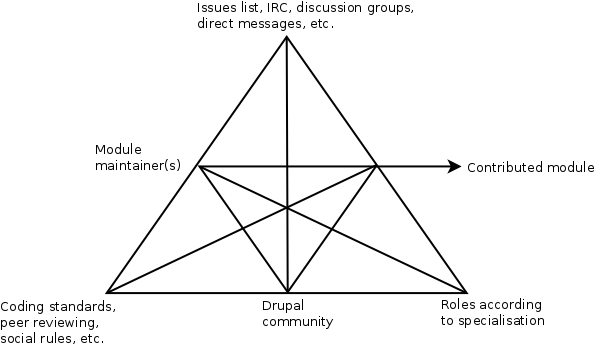
\includegraphics[scale=0.3]{drupal_module_at.png}
	\caption{Conceptualisation of the development of a Drupal contributed module from an AT perspective}
	\label{drupal_module_at}
\end{figure}


\section{Work in progress, expected contributions and expectations}

In the previous example, we have focused on the development of contributed modules. However, a similar approach could be taken to study some other contribution activities, such as the development of core modules, the organisation of F2F events, the translation
processes, the creation of documentation, the activities carried out by the Drupal Association, etc. As part of this process, the ongoing research is looking at the identification of other types of contributions that might be critical for the sustainability of the community (e.g.: to develop a self-identity as a community) beyond the contribution of source code. How these activities are reflected in the collaboration platform and how they are perceived by members of the community with different skills and degrees of experience, are also currently being explored. For example, the organisation of F2F events, and the evangelization of the use of the platform via articles, blogging or social media can be seen as other necessary types of contribution for the sustainability of both the object (software) and the community. Once these activities are identified, a more detailed study of them will be carried out to explore the interactions between the different elements and the connections and tensions between these activities and the others. For example, what are the differences in the dynamics and social practices between the collaboration processes of contributed modules with respect to core ones?

My participation in this Doctoral Symposium would offer a magnificent opportunity to enrich and improve the current research and its mixed-mode approach, thanks to  feedback from the discussion following its presentation if this submission is accepted.


\section{Acknowledgments}
This work was partially supported by the Framework
programme FP7 ICT-2013-10 of the European Commission through project
P2Pvalue (grant no.: 610961).

\bibliographystyle{abbrv}
\bibliography{drupal-cbpp-opensym.bib}


\end{document}